\begin{fullwidth}
    \section{Validators, Trading Fees, \& MEV} \label{sec:validators}

    \begin{adjustwidth}{2cm}{2cm}
        \justify
        A primary concern for dYdX governance in maintaining dYdX Chain will be managing validator incentives. Governance controls the ``fee schedule'', the amount the exchange charges for processing transactions which accrues to validators and stakers. These fees are the primary financial incentive for users to validate and stake on the chain. But validators may also misbehave. This misbehavior may be nefarious: validators may censor or reorder transactions for a profit-a concept known as Maximal Extractable Value, or MEV. This misbehavior may also be a product of a genuine mistake or negligence, such as server downtime leading validators to not process enough blocks. In either case, governance must choose appropriate punishments to disincentivize undesirable behavior. In this section, we discuss what the relevant on-chain parameters are, and what additional actions governance may take, to keep validators aligned with the protocol's best interest.
    \end{adjustwidth}
    
    \textcolor{gray}{\rule{\linewidth}{0.1mm}}
    
\end{fullwidth}

    On August 2023 the dYdX Foundation posted \bhref{https://dydx.forum/t/a-take-on-good-practices-for-dydx-chain-validators-and-stakers/978}{A Take on Good Practices for dYdX Chain Validators and Stakers}. The post provides a guide for the dYdX community on what behaviors are required, acceptable, and unacceptable for validators and stakers on dYdX Chain. These range from relatively obvious guidance, such as ``dYdX Chain validators should not engage in MEV activities'', to more nuanced recommendations regarding specific key-management systems and bare-metal setups. 
    \sidenotequote{A non-exhaustive list of parameters that governance will be able to adjust includes: 
    \begin{itemize}
        \item Add new markets 
        \item Adjust parameters of a live market
        \item Remove any market
        \item Edit the list of 3rd party price sources that the exchange uses
        \item Fee schedule
        \item Trading rewards mechanics
        \item x/distribution module parameters affecting trading and gas fees
        \item x/staking module parameters
        \item Funding rate formula
        \item Control of the insurance fund
    \end{itemize}
    }{\bhref{https://dydx.exchange/blog/v4-deep-dive-governance}{v4 Deep Dive: Governance}}

    Throughout this section, we will be discussing the mechanisms and parameters that v4 governance controls, and may wield to keep validators aligned with the protocol's best interests. 
    
    As we will show, making changes to these parameters and enforcing manual slashing are delicate processes that require an expert understanding of the dYdX ecosystem and its various parties. Being overly aggressive in slashing a validator might spook other validators away from dYdX Chain, whereas not being aggressive enough might encourage additional bad behavior. Therefore, it might be appropriate to form a subDAO of sophisticated community members to adjudicate or review these decisions. Such was the justification for the formation of a ``Slashing Review Committee'', \bhref{https://dydx.forum/t/discussion-protection-against-mev-on-dydx-v4/951}{proposed} by Carl, Myles, and Derek from Reverie, a crypto investment firm that has historically contributed to the dYdX ecosystem and managed its grants program.

    \subsection{Validator Overview}

        We have briefly overviewed the job of a validator in Section \ref{sec:introduction}. Validators are in charge of listening to orders submitted by the chain's users and gossiping those orders to other validators. One validator is selected as the current block proposer, they plug all new orders into their in-memory order book and run the chain's canonical matching engine, finally producing a block that they socialize to other validators. Once two thirds of the chain's validators (by stake weight) have signed-off on the newly proposed block, it is committed to the chain. 

        This process is repeated every few seconds, and requires significant resources from validators to monitor their node's performance and ensure that they are abiding by operational and security best practices. Software or hardware bugs, for instance, could create congestion on the chain, delaying or potentially censoring transactions. Validators must therefore be remunerated for ensuring the chain is operated smoothly, and they must be punished if they fail to do so, whether intentionally or unintentionally.

    \subsection{Positive Incentives: Trading Fees} \label{subsec:tradingfees}

        When users submit orders to buy or sell an asset on dYdX Chain they do not pay any fees, conventionally known as ``gas fees'' to validators and stakers. Instead, users pay a trading fee when their order is matched with a counterparty and a transaction is executed. This fee is a percentage of the size of their order. For example, if a user submits an order to buy \$100 USD worth of BTC-PERP and their trading fee is $0.1\%$, they will pay 10 cents in trading fees to validators if their entire order is filled. This fee is distributed roughly \textit{pro rata} across all active validators on the chain. Each validator takes a commission on their earnings, say $10\%$, and then distribute the remainder to their stakers. 

        \subsubsection{Genesis Parameters}

            The chain's initial fee schedule, along with all other of its initial parameters, are defined during the chain's \textit{Genesis} at the Genesis transaction, or \texttt{gentx}. At a high level, \texttt{gentx} defines the chain's initial markets, accounts, token allocations, and protocol-wide parameters. This includes many of the governance-controlled parameters that we will be discussing for the remainder of the report. Following Genesis, governance may then choose to modify these parameters, submit transactions from community-owned accounts, and add or remove perpetual markets. 

            Parameters are controlled by governance through \texttt{ParameterChangeProposals}. Many of these parameters are described in detail in one of dYdX Trading's latest \bhref{https://dydx.exchange/blog/v4-rewards-and-parameters}{announcements}, and include the various parameters pertaining to validator incentives. 

            We provide an example for querying dYdX Chain's genesis state in Appendix \ref{app:genesis}. We query a dYdX v4 testnet's  \texttt{genesis.json} file using an RPC node provided by \bhref{https://www.allthatnode.com/}{AllThatNode}, a dYdX Chain validator. The \texttt{genesis.json} file contains all of the parameters and chain state variables discussed in this report.

        \subsubsection{Taker and Maker Fees, and Rebates}

            \begin{figure}[htp]
                \centering
                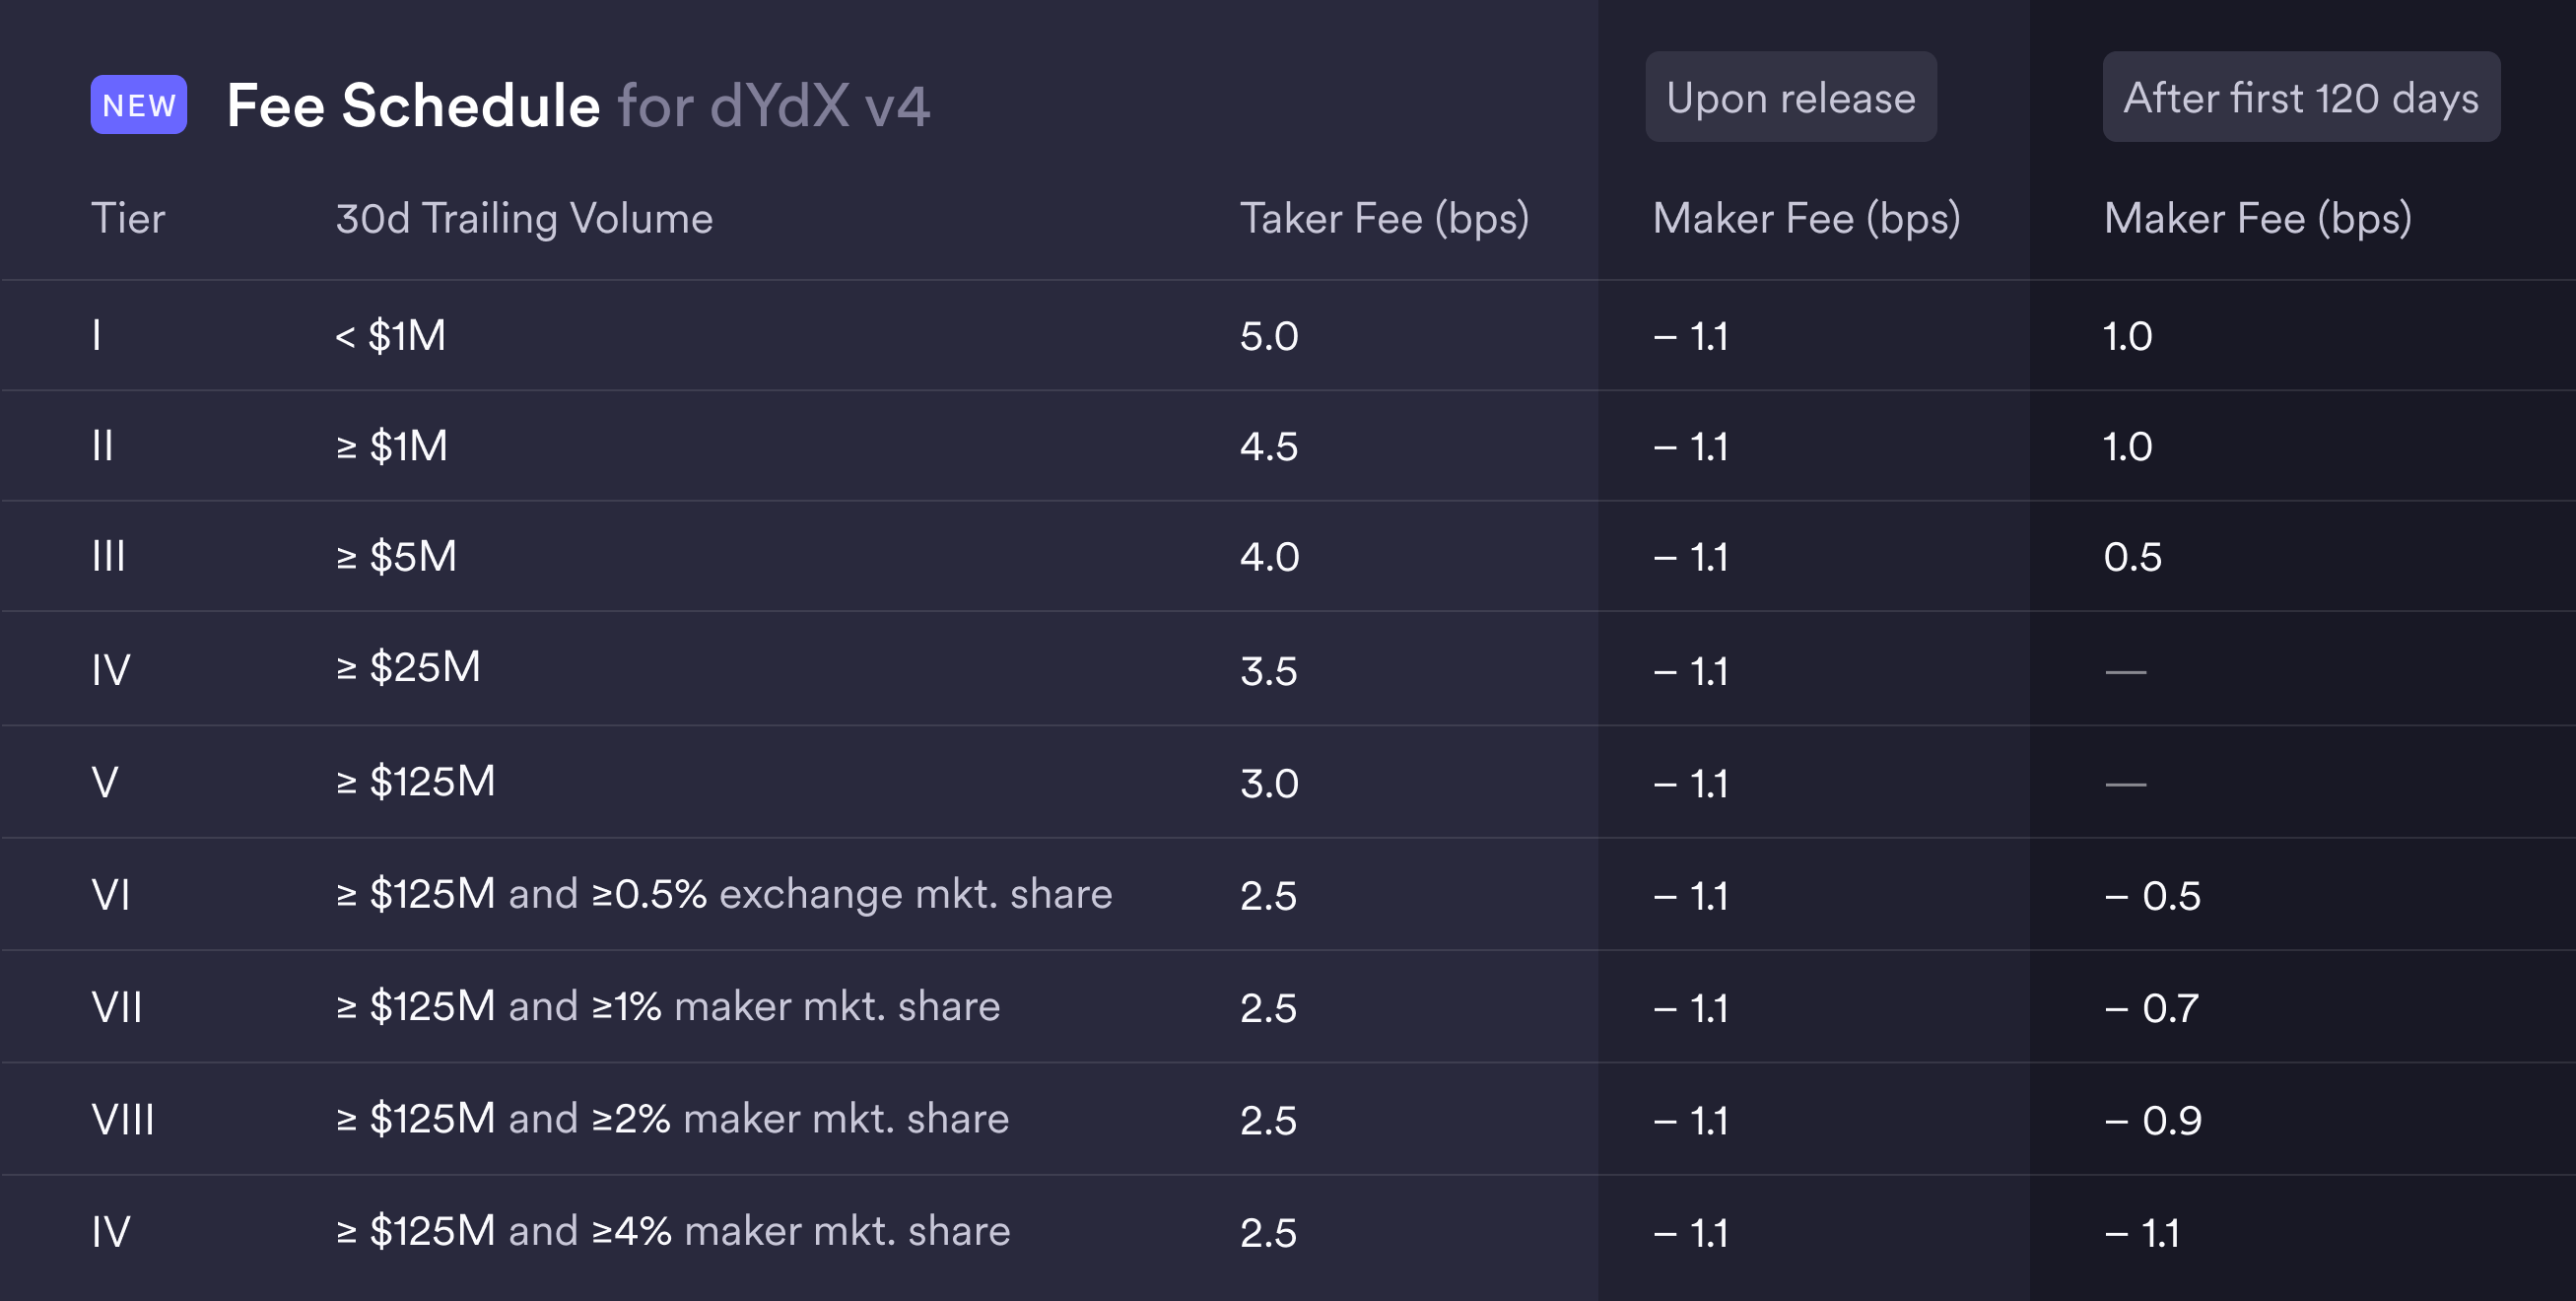
\includegraphics[width=0.7\linewidth]{figs/fees_schedule.png}
                \caption{dYdX Chain fee schedule at Genesis.}
                \label{fig:schedule}
            \end{figure}

            The fee schedule at Genesis is depicted in Fig. \ref{fig:schedule}. Notice that for both makers and takers, fees will decrease as the trader pushes more volume. This is industry-standard scheme is meant to incentivize greater trading volume and, therefore, more liquid markets. For the first 120 days following Genesis, all makers will be receiving a $1.1$bp rebate on their fill size, taken from the fees paid by the taker. That is, all traders submitting limit orders instead of market orders will receive part of their notional in a rebate if their order is filled. Following the 120 day mark, the fee schedule for makers will be changed according to the schedule shown in Fig. \ref{fig:schedule}. Small makers will begin paying a small fee to fill their orders, whereas large makers will continue to receive a rebate.\sidenotequote{Su (2020) highlighted the asymmetric information of existing markets as takers have more information through their willingness to actively remove liquidity from the order book. In contrast, makers are subject to price risk with their idle orders, incurring ‘costs of liquidity’ due to this adverse election on bad fills. As a result, maker rebates appear justified for the tail risks incurred by market makers.}{\bhref{https://drive.google.com/file/d/1g5te0E0jo76UvJw_lbmw5pvqSDJ6HtQd/view}{Trading Fees Optimization Research by 0xCLR and 0xCchan}}

            Of course, all of these parameters, including the 120 days cliff, may be adjusted by dYdX governance. Modifying the fee schedule is a delicate process with material consequences for price-sensitive takers and makers, and must take several factors into account. These factors may include the elasticity of takers and makers at different volume strata, the fees charged by other exchanges, and the demands of the chains stakers and validators for additional fee income. 

            In all likelihood, different parties might submit proposals to either raise or lower fees on dYdX Chain. Market makers, for instance, may wish to lower maker fees to make their operations more profitable and to ensure greater liquidity provision on the exchange. Validators may wish to raise taker and maker fees to ensure they can profitably operate the exchange.

            A common framework for decentralized exchanges to set their fees is to follow trends on larger, centralized exchanges such as Binance. Such a comparison was posted with regards to dYdX v3's fee schedule by Wintermute governance in \bhref{https://dydx.forum/t/drc-adjusting-maker-taker-fees/39}{this} dYdX Request for Comment (DRC).

            \begin{figure}[htp]
                \centering
                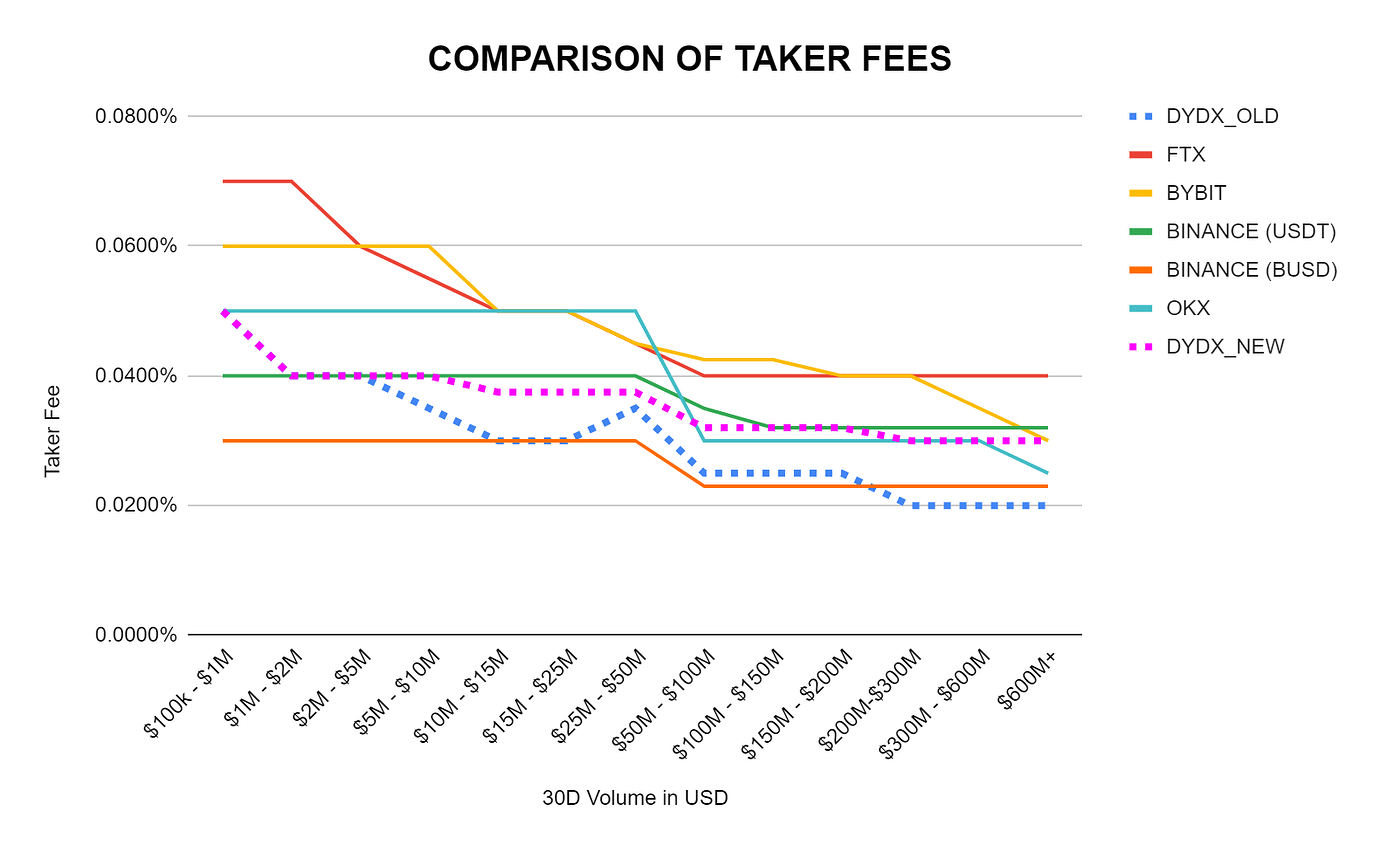
\includegraphics[width=0.7\linewidth]{figs/fee_comp_takers.png}
                \caption{Comparison of Taker fees across crypto exchanges. \bhref{https://dydx.forum/t/drc-adjusting-maker-taker-fees/39}{Source}.}
                \label{fig:fee_comp_takers}
            \end{figure}

            Going into v4, sophisticated community members may wish adjudicate such proposals by discussing them with both makers and takers, as well as the exchange's validators and stakers. They may compare the existing fee tiers with those of other exchanges and determine reasonable modifications, if any. Crucially, changes to such parameters may then be monitored, with these results being used as evidence in later proposals. 
            
            The interested reader may refer to:
            \begin{itemize}
                \item \bhref{https://drive.google.com/file/d/1g5te0E0jo76UvJw_lbmw5pvqSDJ6HtQd/view}{This} research paper published by dYdX community members 0xCLR and 0xCchan on optimizing dYdX's trading fees.
                \item \bhref{https://dydx.forum/t/drc-shifting-from-lp-rewards-toward-market-maker-rebates/594}{This} proposal from Xenophon Labs to transition away from LP rewards and towards market maker rebates.
                \item \bhref{https://dydx.forum/t/passed-snapshot-drc-introduce-a-market-maker-rebate-program/42}{This} proposal from Wintermute governance to introduce market maker rebates.
                \item \bhref{https://dydx.forum/t/drc-adjusting-maker-taker-fees/39}{This} proposal from Wintermute governance to adjust maker and taker fee schedules.
            \end{itemize}

        \subsection{Rebates or Rewards?}

            dYdX v4 will be entirely replacing the LP rewards program, introduced by the dYdX Foundation in dYdX v3, with a market maker rebate program. As noted in a number of governance proposals, market maker rebates are likely a better incentive for top-of-book liquidity, and provide a more sustainable incentive for liquidity provision. That is, they don't require further inflation to the DYDX token.
            
            We invited \bhref{https://dydx.forum/u/0xcchan/summary}{@0xCchan}, a dYdX community member, to offer further insights on the differences between LP rewards and rebates:

            \begin{displayquote}
                The LP Incentive Programme was implemented to encourage MMs to continuously provide two-sided liquidity to markets through rewards. A previous review on the state of the orderbook was done in May 2023, alongside suggested schemes and mechanisms proposed. With the decentralisation of the orderbook, Xenophon Labs has highlighted that the ‘true state’ of it will not be clear and hence different metrics such as depth, spread and uptime will be more challenging to monitor. Therefore, we would need to rely less on orderbook-driven data and shift to clearly defined metrics.

                The most straightforward mechanism would be a rebates solution, where LPs are proportionately rewarded based on the volume churned. This can be easily computed based on on-chain transaction data, where necessary. 

                We may compare a rebates mechanism against the previous LP rewards scheme (prior to the 50\% reduction) by looking at the dollar value of either incentive, shown in Table \ref{tab:lp_rewards_vs_rebates}.

                \begin{table}[htp]
                    \centering
                    \begin{tabular}{l r r r}
                        \toprule
                        & Volume (Rounded Up)	& Rebates (0.5\%) & Rewards (@\$2 USD) \\
                        \midrule
                        BTC / ETH & \$25B & \$125M & \$0.46M \\
                        Altcoins & \$7B	& \$35M	& \$1.84M \\
                        \bottomrule
                    \end{tabular}
                    \caption{Comparison between the dollar value of LP rewards and market maker rebates.}
                    \label{tab:lp_rewards_vs_rebates}
                \end{table}

                Evidently, LPs receive significantly more in rebates than the present level of rewards, with BTC and ETH attracting a disproportionately larger amount (even with the new maker fee structure). Given the resiliency of these 2 markets, a consideration would be then to lower the rebates in the long run, while enhancing the rebates for altcoins. 
            \end{displayquote}

        \subsection{The Community Tax}

            As previously mentioned, fees are first paid to validators, who take a commission and then distribute remaining proceeds to their respective stakers. The community may choose to enforce an additional tax on fee income, which applies before fees are disbursed to validators. This tax, known as the Community Tax, will be set to 0\% at Genesis.

            The community may choose to enforce such a tax to fund additional efforts to grow, secure, or maintain dYdX Chain. As it stands, governance already has tens of millions of dollars in capital to deploy for such efforts, with millions more vesting into the community treasury every month. 

            However, as mentioned in Section \ref{sec:introduction}, the DYDX vesting schedule is set to terminate on August 2026. At this point, no more DYDX will vest into the community or rewards treasuries. If and when the DYDX sitting in the community treasury runs out, the community will be faced with two options to continue funding operations and rewards programs:

            \begin{enumerate}
                \item Enable up to 2\% in annual inflation of the DYDX token.
                \item Enable the community tax on fees on dYdX chain.
            \end{enumerate}

            The community tax is arguably a more sustainable source of funding for the community than enforcing an inflationary schedule on DYDX, but both options are available to the community when the time comes. Until then, there might be other reasons that governance chooses to enforce a tax. For example, a tax might be used to sustainably fund new incentives programs throughout the dYdX Chain ecosystem, such as incentives for front end or indexer operators. We discuss this in Section \ref{sec:feip}.

    \subsection{Negative Incentives: Slashing, \& Jail} \label{subsec:mev}

        There are several mechanisms in place to disincentivize validators from misbehaving, which we place into three general buckets:

        \begin{itemize}
            \item Automatic punishments: jailing, tombstoning, and partial slashing for extended downtime or double-signing blocks.
            \item Manual slashing: governance proposals to slash validators caught censoring, reordering, or front-running transactions.
            \item Preventative measures: potential mechanisms to prevent certain types of misbehavior altogether, currently in the research and development phase.
        \end{itemize}

        We will discuss each below.

        \subsubsection{Jail, Tombstones, and Automatic Slashing}

            Some misbehavior can be detected automatically on dYdX Chain. These include double-signing blocks, a severe infraction that may cause instability in the network, and downtime, staying too long without signing any blocks leading to congestion and slower block times.  

            In either case, the punishment is enforced automatically, and is parameterized according to Table \ref{tab:punishment_params}.

            \begin{table}[htp]
                \centering
                \captionsetup{justification=centering}
                \caption{Validator Punishment Parameters}
                \begin{tabular}{lr}
                    \toprule
                    Name & Value \\
                    \midrule
                    Signed Blocks Window & \( 12000 \) (5 hrs) \\
                    Min Signed Per Window & \( 20\% \) \\
                    Downtime Jail Duration & \( 60 \) s \\
                    Slash Fraction Doublesign & \( 0 \) \\
                    Slash Fraction Downtime & \( 0 \) \\
                    \bottomrule
                \end{tabular}
                \label{tab:punishment_params}
            \end{table}
            
            Let's examine each type of punishment and its corresponding parameters.

            \begin{itemize}
                \item Slashing. Validators may have their stake slashed and redirected to the community pool. According to the Genesis parameters, if a validator double-signs blocks at a particular block height or fails to sign enough blocks during the specified window, they will not be slashed. That is, the slashing percentages are 0 for both infractions. 
                \item Jailing. Validators may be removed from the ``active validator set''. The active validator set are the validators allowed to propose and sign blocks, and are the only ones eligible to receive fee income. Validators may return to the active set after serving their jail time. If a validator fails to sign enough blocks, they will be jailed for 60 seconds.
                \item Tombstoning. Validators may be permanently removed from the active validator set. Given the severity of a double-signing infraction, validators caught signing two or more blocks at the same block height will be tombstoned.
            \end{itemize}

            \begin{marginfigure}
                \centering
                
\includegraphics[width=\linewidth]{figs/bonk.png}
                \caption{Bonk, go to validator jail.}
                \label{fig:bonk}
            \end{marginfigure}

            Governance may choose to make these parameters more or less aggressive to further disincentivize infractions. If governance observes that validators are failing to sign enough blocks, it may choose to increase the slashing percentage from 0 to a modest amount, such as 5\%. In doing so, governance increases the incentive for validators to maintain appropriate uptime. These changes, of course, might incur significant financial consequences for both validators and stakers, and must be examined and justified by sophisticated community members.

        \subsubsection{An Aside on Reputation}

            Validators fundamentally rely on reputation to scale their operations and profits. Validators generally have low percentages of ``self-stake'', meaning most of the staked tokens they operate with are delegated to them by the chain's stakers. Although there are several factors that affect which validator a staker chooses to stake their tokens with, a primary one is the validator's reputation. A reputable validator that is active in governance and has a history of excellent performance is likely to receive a greater share of staked tokens. 

            Conversely, a validator caught engaging in detrimental behavior to the chain, such as censoring, reordering, or front-running transactions is unlikely to receive much in staked tokens. That is, if the broader community is made aware of their infractions. It follows that a major tool dYdX governance has against a misbehaving validator is publicity: publicly announcing a validator's misbehavior may cause them significant financial damage. 

        \subsubsection{MEV \& Social Slashing}

            Perhaps one of the most pervasive opportunities for misconduct on dYdX Chain is MEV, or Maximal Extractable Value. For dYdX Chain, let us define MEV as any value extracted by validators or their co-conspirators by censoring, re-ordering, or front-running transactions. 

            Skip Protocol, in partnership with dYdX Trading's Research team, has produced the following scheme to detect and measure MEV activity from the current block proposer. The idea is simple but effective: any MEV activity will, in some way or another, re-direct profit (or loss) from one account to another. Mathematically, we can express the MEV extracted from a particular block as:

            \begin{equation}
                MEV = \frac{1}{2}\sum_{i}^{N}{|PNL_i^{BP} - PNL_i^{V}|},
            \end{equation}

            where $i$ indexes the $N$ sub-accounts on the chain, and $PNL_i$ is account $i$'s profit or loss at the end of the block. The superscript $BP$ indicates that this is the actual $PNL$ according to the transactions submitted by the block proposer, whereas $V$ indicates the $PNL$ that an ``honest validator'' would have expected.

            The premise of the honest validator is simple: a node that runs the chain's canonical matching engine and does not engage in any MEV. This node, which doesn't need to participate in consensus and can simply be listening to new orders, will construct a block without engaging in any dishonest behavior. This node then compares the $PNL$ at the end of the block with the $PNL$ at the end of the block proposer's block. Any discrepancy may be the result of MEV activities. 

            Given this logic, Skip has built a dashboard that tracks this MEV metric across all validators by comparing blocks to those built by its own honest validator. You may find the dashboard \bhref{https://dydx.skip.money/}{here}, or refer to the screenshot below.

            \begin{figure}[htp]
                \centering
                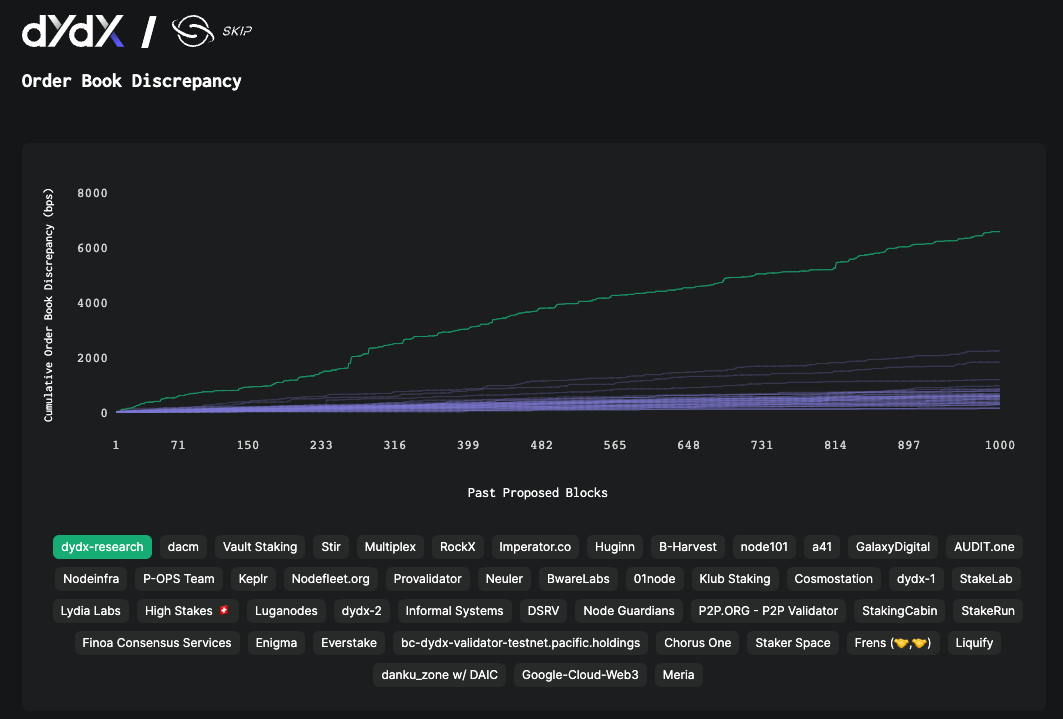
\includegraphics[width=0.7\linewidth]{figs/mev.png}
                \caption{Screenshot of Skip's MEV dashboard taken from \bhref{https://dydx.exchange/blog/update-on-mev}{this} announcement by dYdX Trading.}
                \label{fig:mev}
            \end{figure}

            Leveraging this dashboard and detection algorithm, community members may monitor validators and punish those found engaging in MEV. However, discrepancies seen on the dashboard don't necessarily mean a validator purposefuly censored, re-ordered, or front-ran transactions.

            Consider the case where two buy orders or similar sizes on the same market are submitted roughly at the same time. This is not a rare occurrence: updates to the orderbook may create arbitrage opportunities that two or more traders notice and try to take advantage of. Validators receiving these orders will match them on a first-come-first-serve basis against existing orders. However, it is possible that two honest validators will receive each order at different times. Suppose order $A$ is submitted from Brazil, and order $B$ is submitted from Japan. A validator in South America might receive order $A$ first, whereas a validator in Asia might receive order $B$ first. This is a simple example of a concept known as \textit{network jitter}: the natural discrepancy between when an order is transmitted and when it is received.

            Due to network jitter, honest validators may exhibit non-zero MEV measurements! Therefore, an important task for those punishing dishonest validators is to adjudicate, within reason, when observed discrepancies can be written off as network jitter, and when they are likely the consequence of malicious behavior.

            If community members, such as the potential Slashing Review Committee, determine that a particular validator has engaged in MEV, they may propose to slash this validator. This is known as Social Slashing, and is a severe punishment for the validator. The community may choose to slash part or all of the validator's stake, affecting not only the validator but also the staker. For this reason, stakers must be careful to stake their DYDX with validators that they trust, or risk being slashed.

            One potential tool to distinguish between natural and unnatural MEV measurements is to track the average MEV across all validators, or to run multiple separate ``honest validators'' and compare their MEV between each other. Based on these baseline measurements, MEV that is several standard deviations higher than the baseline may be deemed malicious and result in slashing.

            % \begin{figure*}
            %     \centering
            %     \captionsetup{justification=centering, width=0.8\linewidth}
            %     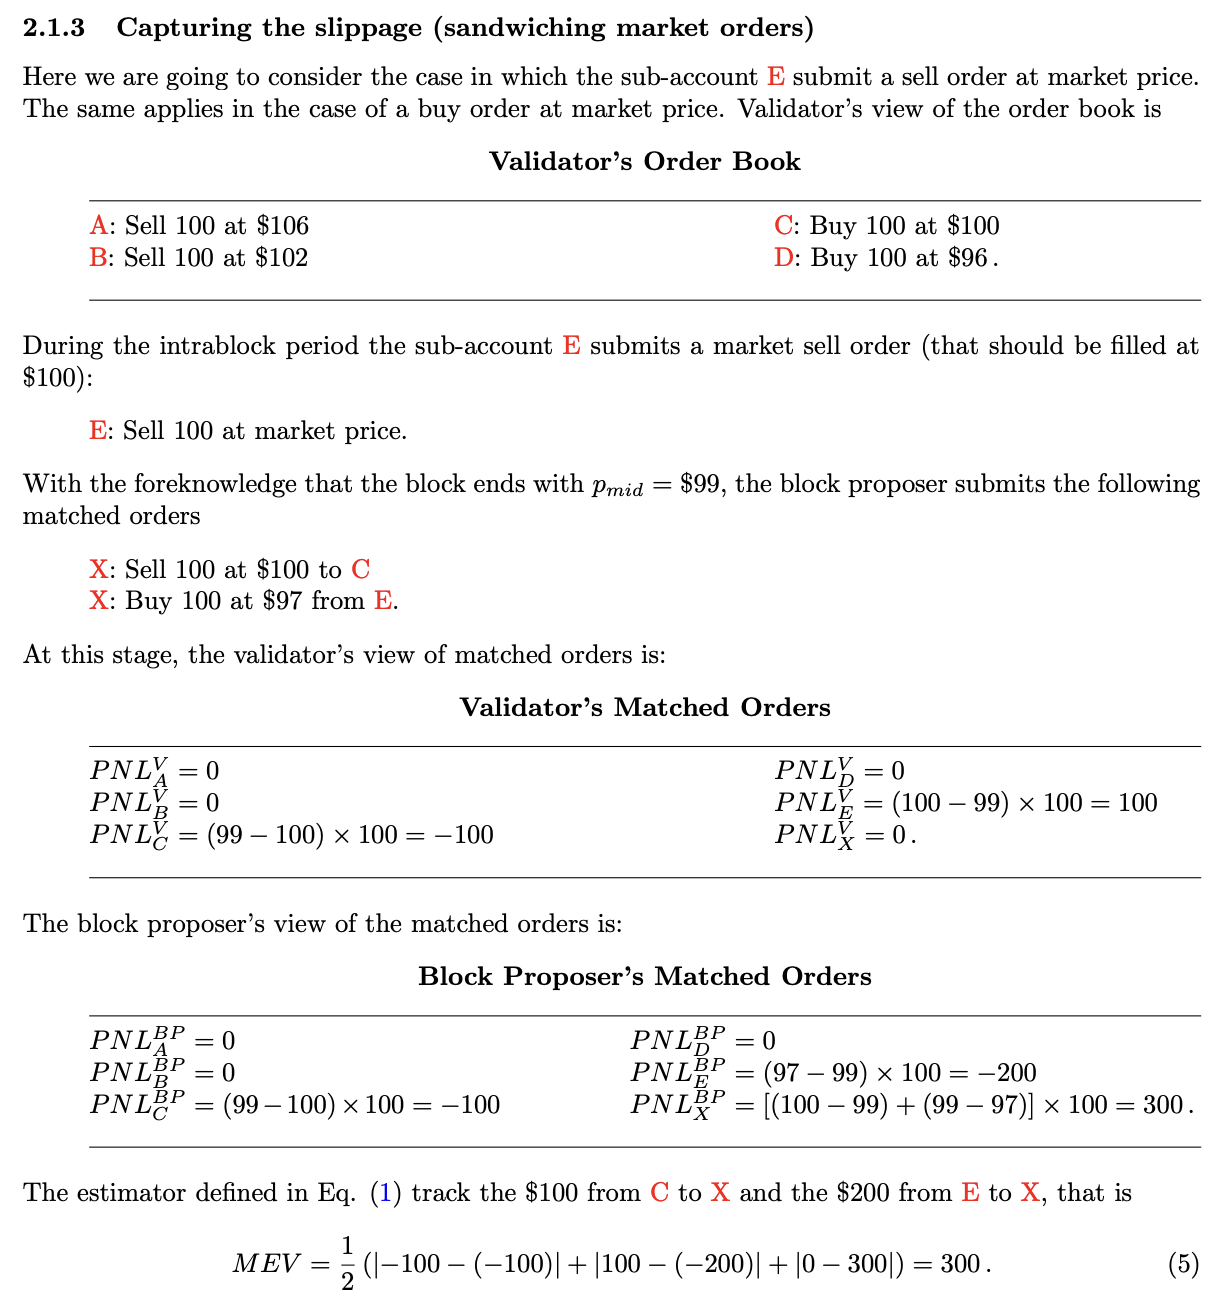
\includegraphics[width=0.8\linewidth]{figs/chorus_one_mev.png}
            %     \caption{A screenshot of Chorus One's MEV \bhref{https://chorus.one/reports-research/mev-on-the-dydx-v4-chain}{report}. This excerpt shows an example of how a validator may perform a \textit{sandwich attack} on a dYdX trader by strategically inserting and re-ordering transactions, and how the MEV detection algorithm would quantify the resulting discrepancy.}
            %     \label{fig:chorus_one_mev}
            % \end{figure*}

        \subsubsection{Preventative Measures}

            There are primarily two forms of MEV that may be present in dYdX V4, which we term ``plaintext-conditional''  and ``plaintext-unconditional'' MEV. An example of plaintext-condition MEV is standard blockchain front-running, such as that seen on Uniswap: a  MEV searcher sees an order, they place their own buy order in front (and possibly a sell order behind, in the case of a sandwich), and they profit from the inflated price introduced by the MEV victim's transaction. This form of MEV is commonly viewed as more harmful to users, and we believe this can be resolved via encryption technologies, such as Trusted Execution Environments or Threshold Encryption.

            On the other hand, plaintext-unconditional MEV is MEV that is extracted, without regard to transaction contents. An example of plaintext-unconditional MEV is top-of-block arbitrage, whereby the latency between blocks leads to price dislocation between on-chain venues and the rest of the market, thus creating an arbitrage opportunity. Block proposers can extract this MEV by placing their own orders before others', or by selling the right to exclusive top-of-block trading to a trading entity. This form of MEV is difficult to detect and punish, since doing so requires either a collaborative block construction process, or a method for the network to veto the ordering of transactions in the block constructed by the block proposer. Generally speaking, the former requires formidably large network bandwidth and low inter-validator latency, while the latter requires nondeterministic slashing conditions (e.g., honest and potentially economically irrational majority assumptions). Although plaintext-unconditional MEV is less pernicious to everyday users than plaintext-conditional MEV, it may degrade the profitability of market makers, who are essential agents in the dYdX V4 exchange marketplace. We look forward to listening and contributing to discussions on mitigating MEV in dYdX's future.
            
